\chapter{Deep Network}
\section{Neural network}
\subsection{Neural}
The basic components of the brain is a neuron. For the ordinary man, we have billion neurons in the human nervous system, and they are connected by the billion of synapses. Each neuron receives input signals from its dendrites and procedures output signals along its axon.\\[0.2cm]
In the computational model of a neuron, the signals travel along the axons interact multiplicatively with the dendrites of the other neuron based on the synaptic strength at the synapse. The synaptic strength are learnable and control the strength at influence or inhibitory of one neuron on another. In basic mode, the input signals are summed and compared with a threshold value. If the sum is greater than threshold value, the neuron can fire, sending a spike along its axon. Actually, we have many firing rate (called activation function) at a neuron, and the common choice of activation function is the \textbf{sigmoid funciont $\sigma$}, because it take a real-valued input and squashes it to range between 0 and 1. The image () show the model of a neuron:
\begin{figure}[h]
	\centering
	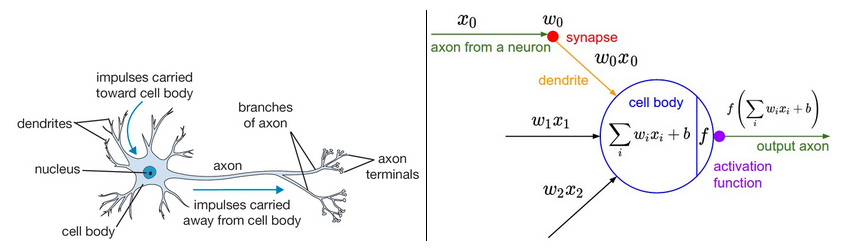
\includegraphics[scale=0.5]{images/neurons.png}
	\caption{A drawing of a biological neuron and its mathematical model}
	\label{fignneuron}
\end{figure}
Some activation functions which we can use:
\begin{itemize}
	\item \textbf{Sigmoid function}:
		\begin{equation}
			\sigma(x) = \frac{1}{1+e^{-x}}
		\end{equation}
	\item \textbf{Tanh}
		\begin{equation}
			tanh(x) = 2\sigma(2x) - 1
		\end{equation}
	\item \textbf{ReLU}
		\begin{equation}
			f(x) = max(0,x)
		\end{equation}
	\item \textbf{Maxout}:
		\begin{equation}
			f(w^Tx + b) = max({w_1}^Tx + b_1,{w_2}^Tx + b_2)
		\end{equation}
\end{itemize}
\section{The architecture of neural networks}
\begin{figure}[h]
	\centering
	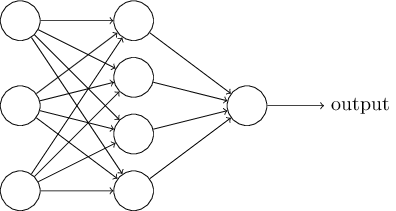
\includegraphics[scale=0.5]{images/neuron}
	\caption{A model of neural networks}
	\label{fignnnetworks}
\end{figure}
The image \ref{fignnnetworks} show a simple model of neural networks. The leftmost layer in this network is called the input layer, the rightmost layer is called the output layer. The neurons within the input layer are called input neurons, the neurons from output layer are called output neurons. The middle layer is called a hidden layer.
\section{Deep network}